\section{How important is the treatment of resources from housing in determining who is poor?}\label{sec:housing}

Section \ref{sec:trends} showed that, in aggregate, adding the imputed resources from housing to measures of household resources (whether income or consumption) increases the apparent growth in living standards over the past 30 years, and reduces the apparent level of inequality.   This section explores how adding the imputed resources from housing changes our impression of which households are in poverty, in a similar way to how Section \ref{sec:compositionwith} explored how moving from income to consumption as our measure of household resources, altered the composition of who is in poverty. 

%[And does something else too?]


\subsection{title needed?}

Table \ref{table:ahc_bhc} reports results of analysis that is analogous to that reported in Table \ref{table:multinom_incon}. Taking income and consumption measures separately, and using data from 1999 to 2009 (with results for other decades in Appendix \ref{sec:annex_results}), we estimate a mutinomial logit for being in one of four groups: (1) in the bottom decile group of the distributions of resources both with and without imputed resources from housing; (2) in the bottom decile group of the distribution without imputed resources from housing but not with resources from housing; (3) in the bottom decile of the distribution with imputed resources from housing but not without; (4) not in the bottom decile group of either distributions.  With ``not in the bottom decile group of either'' as the reference category, we again test for equality of the risk ratios on various observed characteristics of households with different poverty classifications.  In this table, the numbers reported in the 4\nth and 8\nth columns, titled $r_{B}-r_{A}$, are the differences between the risk ratio for being in the bottom decile group of the distribution of resources with imputed resources from housing and the risk ratio for being in the bottom decile group of the distribution of resources without imputed resources; positive values in these columns mean that the characteristic is a stronger predictor of being in the bottom decile group of the distribution of resources with imputed resources from housing than without.

The left-hand panel of Table \ref{table:ahc_bhc} shows that being highly educated, being aged 50 or more, and (especially) being unemployed are all (separately) stronger predictors of being in the bottom decile group of the distribution of income without imputed income from housing than with. In the other direction, being aged 30-40 (compared to age 40-50) [Mike says Abi: where are the cut-points? is it 30-39, 40-49 etc?], and (especially) having a low level of education are both stronger predictors of being in the bottom decile group of the distribution of income with imputed income from housing than without. Viewed another way, this means that when we add the imputed income from housing, the bottom decile group contains fewer households that are aged 50 or more, or highly educated, or unemployed, and more who are aged 30-40, or employed, or with low levels of education. The right-hand panel shows the results for adding the imputed consumption from from housing to the measure of consumption: the results are qualitatively very similar, although the extent to which adding resources from housing changes the age gradient is greater for consumption than it is for income. Overall, the results in Table \ref{table:ahc_bhc} indicate that adding the imputed resources from housing alters the characteristics of those deemed to be poor by giving less weight [wrong phrase] to those more likely to be temporarily poor (the unemployed and those with high education). Adding the imputed resources from housing also reduces the slope of the age profile of poverty.




\begin{sidewaystable}
\caption{Demographics and the Bottom Decile of IHC \& XHC Distributions, 1999-2009: Relative Risk Ratios}
\centering
\begin{tabular}{l|cccc|cccc}
\hline\hline 
	& \multicolumn{4}{c}{\textbf{Income Bottom Decile}} &  \multicolumn{4}{c}{\textbf{Cons. Bottom Decile}} \\
	&	$r_{IX}$	&	$r_{I}$	&	$r_{X}$ &	$r_{I}$-$r_{X}$&	$r_{IX}$	&	$r_{I}$	&	$r_{X}$	&	$r_{I}$-$r_{X}$\\
  & se & se & se  & $\chi^{2}$ & se & se & se & $\chi^{2}$ \\
\hline
Left school $\leq$ 16	&	       1.37***  	&	       2.51***	&	      1.45***	&	1.06****	&	     					  3.17***	&	       2.89***	&	2.79***	&	0.11	\\
                   		 	&	       0.10  	&	0.31	&	0.09	&	18	&	      
						 0.23   	&	0.33	&	0.27	&	0.08	\\
16 $<$ Left school $<=$ 19	&	       0.96   	&	       0.97  	&	1.46***	&	-0.48***	&	
				       1.08   	&	       1.01  	&	       1.78***  	&	-0.78***	\\
                    		&	       0.08   	&	0.09	&	0.14	&	7.8	&	     
					  0.08   	&	0.09	&	0.18	&	24	\\
Age $<$ 30	&	       1.92*** 	&	       1.89***  	&	1.95***	&	-0.06	&	
			       2.07***  	&	1.30***	&	1.84***	&	-0.54***	\\
                    	&	       0.13   	&	0.10	&	0.23	&	0.04	&	  
			     0.17   	&	0.10	&	0.18	&	17	\\
Age 30-40	&	      1.20***   	&	       1.44***	&	       0.99 	&	0.45***	&	
			       1.34***   	&	       1.26***	&	1.08	&	0.18***	\\
                    	&	       0.05   	&	0.10	&	0.09	&	9.5	&	  
			     0.07   	&	0.06	&	0.06	&	3.7	\\
Age 50-60	&	       0.63***	&	       0.36***	&	0.84***	&	-0.48***	&
			       0.56***	&	       0.43***	&	       0.96 	&	-0.54***	\\
                    	&	       0.02   	&	0.07	&	0.05	&	15	&	
			       0.03   	&	0.03	&	0.09	&	54	\\
Age 60-70	&	       0.16***	&	       0.17***	&	       0.27***	&	-0.10***	&	       								0.22***	&	       0.23***	&	0.53	&	-0.31***	\\
                    	&	       0.01   	&	0.02	&	0.02	&	8.4	&	
			       0.02   	&	0.02	&	0.04	&	97	\\
Age $\geq$ 70	&	       0.09***	&	       0.15***	&	       0.25***	&	-0.10***	&	    					   		0.51***	&	       0.30***	&	       1.15 	&	-0.85***	\\
                    	&	       0.01   	&	0.02	&	0.03	&	7.5	&	    
				   0.05  	&	0.03	&	0.12	&	225	\\
Workless	&	       14.7***	&	       11.7***	&	       16.1***	&	-4.47***	&	       					11.9***	&	      5.20***	&	       8.04***	&	-2.85***	\\
	&	       0.81   	&	0.91	&	1.05	&	8.1	&	
		       0.67   	&	0.50	&	0.28	&	31	\\
Self Employed	&	       3.74***	&	      1.84***	&	       2.82***	&	-0.98**	&	       							0.80***	&	       0.97&	       0.73***	&	-0.24***	\\
	&	       0.34   	&	0.22	&	0.25	&	5.5	&	
		       0.07   	&	0.09	&	0.08	&	7.3	\\
Constant            	&	       0.027**	&	       0.006***	&	0.010	&		&	
				       0.012***	&	       0.010***	&	       0.008***	&		\\
                    	&	       0.002   	&	0.001	&	       0.001 	&		&	 
			      0.001   	&	0.001	&	0.001	&		\\
\hline\hline
\multicolumn{9}{l}{Significantly different from zero at the 10\% ($\star$),  5\% ($\star\star$) and 1\% level ($\star\star\star$).} \\
\multicolumn{9}{l}{Omitted variables: Left school over 19 years old, household head aged between 40 and 50 years, employed. } 
\end{tabular}
\label{table:ahc_bhc}
\end{sidewaystable}

\begin{sidewaystable}
\caption{Demographics and the Bottom Decile of IHC \& XHC Distributions, 1999-2009: Relative Risk Ratios}
\centering
\begin{tabular}{l|cccc|cccc}
\hline\hline 
	& \multicolumn{4}{c}{\textbf{Income Bottom Decile}} &  \multicolumn{4}{c}{\textbf{Cons. Bottom Decile}} \\
	&	$r_{IX}$	&	$r_{I}$	&	$r_{X}$ &	$r_{I}$-$r_{X}$&	$r_{IX}$	&	$r_{I}$	&	$r_{X}$	&	$r_{I}$-$r_{X}$\\
  & se & se & se  & $\chi^{2}$ & se & se & se & $\chi^{2}$ \\
\hline
Left school $\leq$ 16	&	       1.34***  	&	       2.09***	&	      1.49***	&	0.60**	&	     					  2.70***	&	       2.54***	&	2.85***	&	-0.32	\\
                   		 	&	       0.10  	&	0.26	&	0.11	&	6.0	&	      
						 0.23   	&	0.28	&	0.30	&	0.64	\\
16 $<$ Left school $<=$ 19	&	       1.00   	&	       0.85*  	&	1.71***	&	-0.58***	&	
				       0.83   	&	       0.92  	&	       1.78***  	&	-0.79***	\\
                    		&	       0.08   	&	0.08	&	0.14	&	12	&	     
					  0.06   	&	0.08	&	0.17	&	31	\\
Age $<$ 30	&	       1.79*** 	&	       1.95***  	&	1.61***	&	0.34	&	
			       1.83***  	&	1.57***	&	1.51***	&	0.07	\\
                    	&	       0.13   	&	0.19	&	0.18	&	1.4	&	  
			     0.178  	&	0.15	&	0.15	&	0.23	\\
Age 30-40	&	      1.14***   	&	       1.31***	&	       0.91	&	0.40***	&	
			       1.21***   	&	       1.28***	&	1.01	&	0.27***	\\
                    	&	       0.05   	&	0.10	&	0.09	&	8.2	&	  
			     0.06 	&	0.06	&	0.07	&	9.4	\\
Age 50-60	&	       0.71***	&	       0.73	&	0.81***	&	-0.08	&
			       0.78***	&	       0.74***	&	       0.95 	&	-0.21**	\\
                    	&	       0.03   	&	0.16	&	0.07	&	0.1	&	
			       0.05   	&	0.05	&	0.09	&	4.9	\\
Age 60-70	&	       0.19***	&	       0.57***	&	       0.23***	&	0.34***	&	       								0.37***	&	       0.60***	&	0.50***	& 0.10**	\\
                    	&	       0.02   	&	0.07	&	0.02	&	19	&	
			       0.03   	&	0.04	&	0.09	&	4.7	\\
Age $\geq$ 70	&	       0.10***	&	       0.54***	&	       0.17***	&	0.37***	&	    					   		0.79**	&	       0.86***	&	      0.90 	&	-0.04	\\
                    	&	       0.01   	&	0.06	&	0.02	&	30	&	    
				   0.08  	&	0.07	&	0.12	&	0.47	\\
Workless	&	       12.5***	&	       10.3***	&	       11.9***	&	-1.64	&	       									9.42***	&	      5.16***	&	       5.35***	&	-0.20***	\\
	&	       0.69   	&	0.89	&	0.73	&	1.4	&	
		       0.51   	&	0.50	&	0.19	&	0.15	\\
Self Employed	&	       3.88***	&	      1.69***	&	       3.41***	&	-1.72***	&	       							0.81**	&	       0.90 &	       0.89	&	0.01	\\
	&	       0.35   	&	0.21	&	0.31	&	14	&	
		       0.07   	&	0.09	&	0.09	&	0.03	\\
Couple	&	       0.87	&	      0.68***	&	       1.53***	&	-0.84***	&	       							0.68***	&	       0.58*** &	       1.09	&	-0.52***	\\
	&	       0.07  	&	0.08	&	0.16	&	40	&	
		       0.05   	&	0.05	&	0.17	&	14	\\
Single	&	       1.66***	&	      0.92	&	       6.46***	&	-5.55***	&	       							1.59***	&	       0.60***&	      6.66*** &	-6.05***	\\
	&	       0.14   	&	0.12	&	0.71	&	297	&	
		       0.13   	&	0.04	&	1.04	&	239	\\
Child Dummy	&	       1.27***	&	      5.36***	&	      0.72***	&	4.64***	&	       							2.09***	&	       3.80*** &	       0.77***	&	3.04***	\\
	&	       0.09   	&	0.59	&	0.06	&	289	&	
		       0.10   	&	0.22	&	0.06	&	378	\\
Constant            	&	       0.023**	&	       0.003***	&	0.004***	&		&	
				       0.010***	&	       0.006***	&	       0.004***	&		\\
                    	&	       0.002   	&	0.001	&	       0.001 	&		&	 
			      0.001   	&	0.001	&	0.001	&		\\
\hline\hline
\multicolumn{9}{l}{Significantly different from zero at the 5\% ($\star\star$) and 1\% level ($\star\star\star$).} \\
\multicolumn{9}{l}{Omitted variables: Left school over 19 years old, household head aged between 40 and 50 years, employed. } 
\end{tabular}
\label{table:ahc_bhc}
\end{sidewaystable}


\subsection{title needed?}

The results discussed above show that adding the imputed resources from housing reduces the slope of the age profile of poverty.  Figure \ref{fig:pov_age} probes this result more, by showing the age profile of being in the bottom decile group of [Mike asks Abi: is this income or consumption? Could we have both?] for different birth cohorts with and without the imputed resources from housing. The key points are as follows. First, however measured, the age profile of poverty is becoming less steep for successive birth cohorts. [Mike asks Abi: some of the numbers in the figures are very low - just a $2\%$ chance of being in the bottom decile? Also, I am concerned that some of these look q different from Figures 40-42 of the Brewer-O'Dea WP.] This is in line with findings in [XXXX] that old age is no longer a good predictor for being in the poorest group (although they confound age and cohort). More importantly for our analysis, though, is that the age profile of being in the bottom decile group of income/consumption [which?] including imputed resources from housing is becoming increasingly less steep over time than the age profile of being in the bottom decile group of income/consumption without imputed resources from housing. Indeed, for the 1950s cohort, the age profile  of being in the bottom decile group of income/consumption with imputed resources from housing is broadly flat (at least after the late 30s), whereas it remains upward sloping (at least above age 40) when resources are measured without those from housing.

[Mike asks ABi and COrmac: I still find myself wanting to show how the cohort-profile of poverty in a given year as changed over time (as we did in the WP). Can we? please?]

Clearly, many of these results are due to the age- and cohort- patterns in the ownership of housing, and the value of that implicit consumption or income that home-owners enjoy. Panel (a) of Figure \ref{fig:room_age_tenure} shows the fraction of individuals/households [which?] who live in owner-occupied housing by age and cohort. The life-cycle pattern is unsurprising, with home-ownership rising steeply between mid 20s to the mid 40s, and more slowly thereafter. But the figure also reveals the striking cohort patterns: for a given age, home-ownership is the most likely for the 1940s and 1950s cohorts, and less likely for all others.  [Mike asks Abi: are these raw data? Smoothed? from an APC analysis? we probably need to give detail on how these were created or smoothed etc].

Panel (b) of Figure \ref{fig:room_age_tenure} does a similar analysis for the number of rooms [Mike asks Abi: precise definition?] occupied by households who own their own house [Mike asks Abi: is this right? i.e is it conditional on owning a property?]. [Mike asks Abi and Cormac: I am not sure what it shows. And we discussed that there seems to be a time effect, in that all cohorts see a fall in number rooms in 2000. We noted this when we met, and I have an email (sent by me 13/03/2015) saying that Cormac was going to look at this, but I don't have a record of the answer].


\begin{figure}
\caption{Risk of Poverty, by Age and Cohort }
\centering
\begin{tabular}{c c}
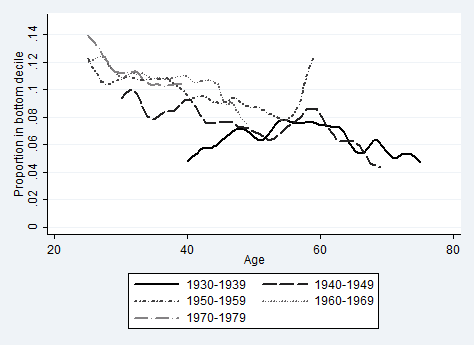
\includegraphics[width=.5\linewidth]{pictures/cohortagerisksmooth_bhc_inc.png} &
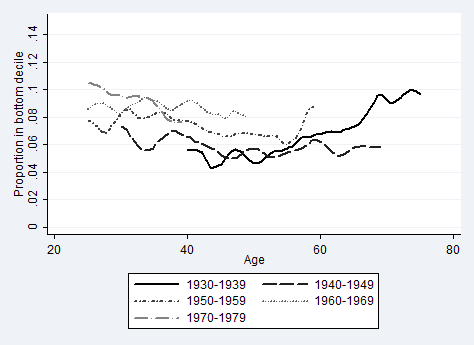
\includegraphics[width=.5\linewidth]{pictures/cohortagerisksmooth_bhc_con.png} \\
(a) Income inc. Housing & (b) Consumption inc. Housing \\
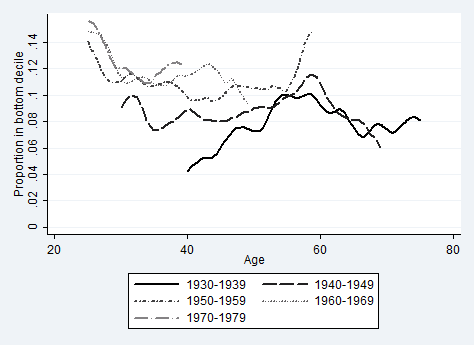
\includegraphics[width=.5\linewidth]{pictures/cohortagerisksmooth_ahc_inc.png} &
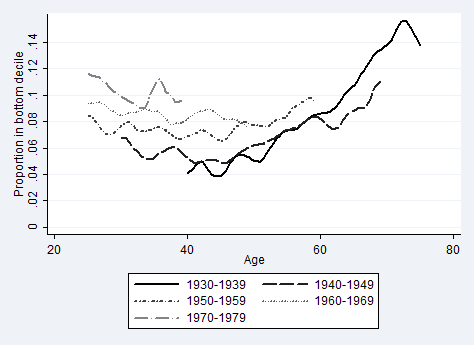
\includegraphics[width=.5\linewidth]{pictures/cohortagerisksmooth_ahc_con.png} \\
(c) Income ex. Housing & (d) Consumption ex. Housing \\
\end{tabular}
\label{fig:povage_cohort}
\end{figure}

\begin{figure}
\caption{Risk of Poverty, by Age and Cohort }
\centering
\begin{tabular}{c c}
Income & Consumption\\
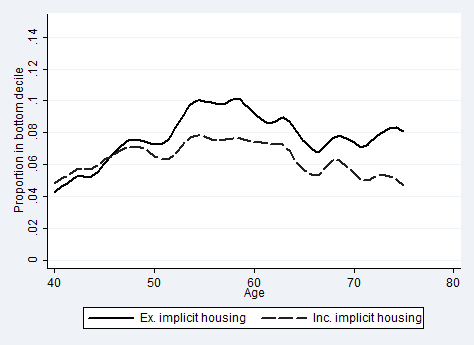
\includegraphics[width=.5\linewidth]{pictures/cohort2_agerisksmooth_inc.png} &
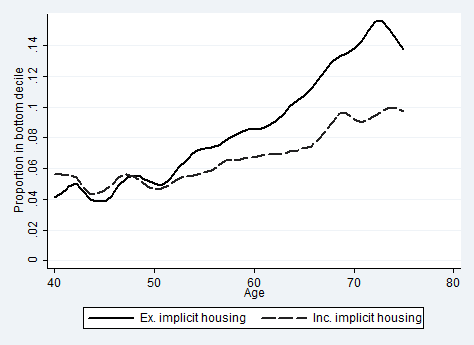
\includegraphics[width=.5\linewidth]{pictures/cohort2_agerisksmooth_con.png} \\
(a) 1930s Cohort & (b) 1930s Cohort \\
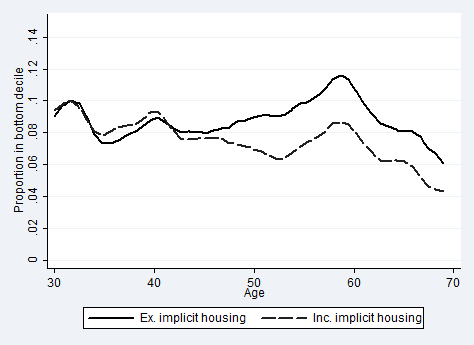
\includegraphics[width=.5\linewidth]{pictures/cohort3_agerisksmooth_inc.png} &
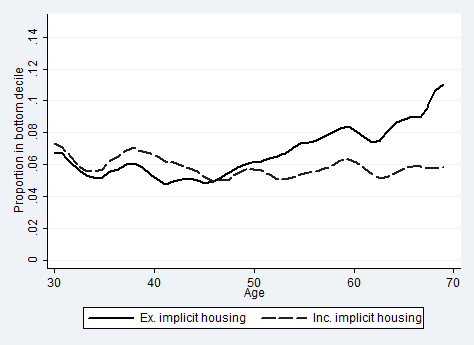
\includegraphics[width=.5\linewidth]{pictures/cohort3_agerisksmooth_con.png} \\
(c) 1940s Cohort & (d) 1940s Cohort \\
\end{tabular}
\label{fig:povage_cohort_restrict}
\end{figure}


\begin{figure}
\caption{Average Rooms Occupied per Person}
\centering
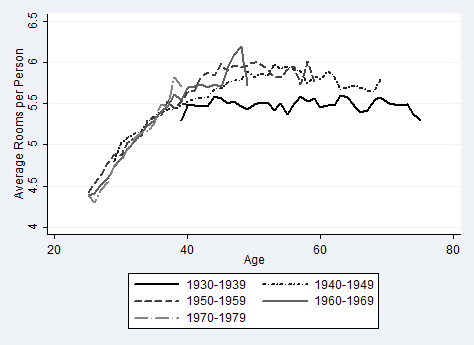
\includegraphics[width=.7\linewidth]{pictures/cohort_rooms.png}
\label{fig:cohort_rooms}
\end{figure}

\begin{figure}
\caption{Average People in Household}
\centering
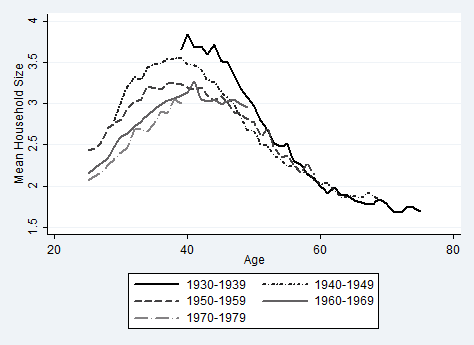
\includegraphics[width=.7\linewidth]{pictures/av_peep.png}
\label{fig:cohort_peeps}
\end{figure}


